\chapter{k8-resource-optimizer}
\label{ch:k8-bench}
This chapter presents the architecture and implementation of k8-resource-optimizer, an automated SLA-decomposition tool for Kubernetes applications. The k8-resource-optimizer allows to create a SLO-decomposition for a particular application given a workload and tenant configuration. The first section of this chapter briefly revisits the problem statement of SLA-decomposition. Next, an overview of the essential requirements for the architecture of the tool is given. The remaining sections discuss the adaption of BestConfig's optimization algorithm for SLA-decomposition and the overall architecture of the tool. 
\section{Motivation}
Today's industry-level SaaS providers face the constant challenge of offering their products at the best service level for the most competitive price.  SaaS providers employ trends such as multi-tenancy and container orchestration in order to meet these agreed-upon SLAs while minimizing resource utilization, thus reducing operating cost. 
For the simple batch processing application, introduced in Chapter~\ref{chapter_app}, the following SLOs are composed:
\begin{itemize}
    \item Bronze tenant:
        \begin{itemize}
            \item Throughput: 0.5 jobs per second
            \item Job size: 250 tasks
        \end{itemize}
    \item Silver tenant:
                \begin{itemize}
                    \item Throughput:  0.5 jobs per second
                    \item Job size: 500 tasks
             \end{itemize}
\end{itemize}

\noindent As discussed in Section~\ref{rw:eddy} resource provisioning policies of container orchestration platforms offer a manner to achieve Quality of Service differentiation. Given a set of SLAs and a service, a provider must translate these SLOs to component level resource requirements. This process is  referred to as SLA-decomposition by~\cite{chen2007sla}. As an example, for the simple batch processing application and an SLO with throughput $T$ and latency $R$, the SLA decomposition task could consist of finding the following mapping:
\begin{equation}
(T,R) \rightarrow (\theta_{cpu-queue},\theta_{mem-queue},\theta_{cpu-worker},\theta_{mem-worker} )
\end{equation}

\noindent However, enterprise SaaS applications have complex architectures consisting of numerous interacting components, making SLA-decomposition a difficult task. Simply finding a configuration that satisfies the SLO does not allow the provider to be competitive, constraints need to be introduced. A common goal is to prohibit \textit{under-provisioning} and to minimize \textit{over-provisioning}. A system is in an over-provisioned state if the amount of allocated resources if greater than the resources required to meet the SLO for the customer. In contrast, a system is under-provisioned when the allocated resources do not suffice to meet the SLOs, resulting in SLA-violation. Under-provisioning a component might potentially result in an unstable system causing high-level characteristics such as availability to become unpredictable.~\cite{al2018elasticity}\\\\
The task of creating a decomposition mapping is often performed by an expert or system administrator relying on their domain knowledge and past experience. A user study on job submissions to a production cluster reported in~\cite{jyothi2016morpheus} shows that 70\% of jobs were over-provisioned and 20\% of them allocated 10x more resources than necessary. This indicates that finding the optimal resource allocations is a hard problem for the average developer. \\\\
In this work, we set out to design a tool for automatically tuning resource allocations for a given SLO and given workload. The next section describes the requirements for such a tool. 
\newpage
\section{Requirements}
The automatic derivation of a resource allocation for a given application and SLO is a complex task which is further complicated by design  decisions such as architecture, underlying technology and deployment. For example, the performance evaluation of a job-oriented service differs from the methodology used for a long-running request-oriented web-service. An application can have a monolithic or microservice architecture. The underlying platform and the deployment strategy also influence the performance characteristics of an application. In sum, the tool should try to fulfill the following requirements:
\begin{itemize}
    \item \textbf{R1:}  Minimal overhead: SaaS applications compromised out of multiple components lead to a multi-dimensional search space for the optimal resource allocations that meet the given SLOs. A configuration should be found with a minimal amount of sampling. In addition, changes or extensions to  commercial applications or the environment in which they are deployed are part of the daily development process. Thus, the overhead added to this process by the tool should be kept to a minimum.
    \item \textbf{R2:}  Versatile: The tool should be able to be configured for a wide variety of architectures and workloads. The architecture could exist of any number of components, each having different components for tuning. Both long-lived workloads and batch workloads should be usable to evaluate the performance of a particular application. 
    \item \textbf{R3:}  Extensible: The architecture of the tool should be extensible. There should be the option to extend to other orchestration platforms, use a different performance evaluation method or employ an alternative for workload simulation.
    \item \textbf{R4:}  Understandable: Most development teams do not have seasoned researchers at their disposal to build complex performance model for their applications. Or the scope of their infrastructure exceeds the scope of systems for which performance models were previously built, such as Hadoop.   The tool should employ a performance  evaluation method that is understandable, trustful and configurable.
    \item \textbf{R5:}  Minimal invasive: The adaptions needed to be made to the applications in order to easily change the configuration need to be kept to a minimum. In the ideal situation, a developer should not alter her/his normal workflow.
    
\end{itemize}
\newpage


\section{Architecture}
\subsection{Overview}
The k8-tool is inspired by the BestConfig application presented in~\cite{zhu2017bestconfig}. As already shortly motivated in the conclusion (Section~\ref{rw:conclusion} of related work, the BestConfig approach is selected over model-based optimization approaches because of its adaptivity towards different applications and understandablity.  The focus of the tool, as derivable from the name, is on Kubernetes applications and incorporates the notion of a \textit{Service Level Objective} that needs to be met utilizing as few resources as possible. It consists of two major components, \textit{SLA-decomposer} and \textit{Bench}. It's architecture is shown in Figure~\ref{fig:k8-architecture}.\\\\ The \textit{SLA-decomposer} is responsible for the translation of Service Level Objects to resource requirements of the various components that make up the Kubernetes application. Its goal is to find the most optimal configuration of resources given an SLO. \\\\
The \textit{Bench}-component actually tests the performance of a given configuration of the Kubernetes application by using a workload simulator, such as a load testing framework. 

\begin{figure}[H]
    \centering
    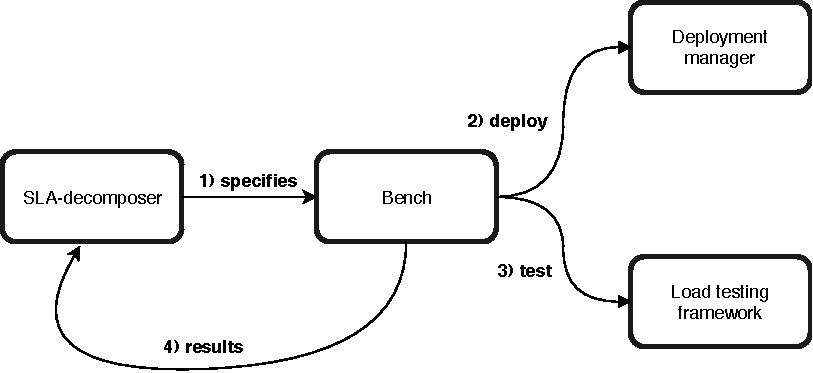
\includegraphics[width=0.8\textwidth]{chapter-k8-bench/k8-bench-architecture.pdf}
    \caption{The architecture of the k8-resource-optimizer tool.}
    \label{fig:k8-architecture}
\end{figure}
\subsection{SLA-decomposer}
The SLA-decomposer employs an adapted version of the performance optimization algorithm used by BestConfig~\cite{zhu2017bestconfig}. The complete algorithm is explained in Section~\ref{rw:bestconfig}. The algorithm consists of three major components:\textbf{ Recursive Bound \& Search} (RBS), \textbf{Divide and Diverge sampling} (DDS) and a \textbf{Utility function}.
The combination of RBS and DDS allows to find the best configuration in a high dimensional parameter space in a limited amount of samples and iterations. Allowing \textbf{R1} to be achievable. A configuration is considered as the best option when it receives the highest score by the utility function.
\subsubsection{Input configuration}
\label{input-config}
Listing~\ref{lst:slaconfig} shows an example of an input configuration for the SLA-decomposer. A configuration consists out of multiple SLAs. Each SLA specifies the following options: Service Level Objectives to be met, amount of tenants and the parameters (resources) to be tuned. For each parameter a search space is defined which restricts the upper and lower bounds of the resource. It is also possible to specify a necessary prefix or suffix for the parameter (e.g., suffix m for 500m CPU). Lastly, a multi-tenant deployment strategy is configured. This is either \textit{Namespace per SLA} or \textit{Namespace per tenant} as described in Section~\ref{rw:eddy}. Also, the number of iterations and number of samples in each iteration for the PO algorithm can be specified.\\\\
Given a configuration the SLA-decomposer will complete the following steps in each iteration:
\begin{enumerate}
    \item Take $x$ samples of each parameter in their current search spaces using DDS.
    \item Create a \textit{Bench} configuration according to the specified deployment strategy, parameter samples and evaluation test(s).
    \item Execute the \textit{Bench} configuration.
    \item Process the results of the evaluation method (specified in \textit{Bench} configuration) to obtain a utility function score for the chosen parameter combinations.
    \item Select the current best parameter combination and perform RBS to obtain the next search spaces for each parameter.
\end{enumerate}
\subsubsection{Utility function}
In BestConfig, the utility function is a scalar function. It translates multiple user-concerned performance goals to a single value. In the case of SLA-composition in which SLOs have to be met with a minimal set of resources we propose the following utility function:
\begin{equation}
   $$
\[ f([]SLOmetrics, []resoureLimits) = 
  \begin{cases}
    0      &  \text{ SLA is violated}\\
    \sum_{r=1}^{len(resoureLimits)} (1 - \frac{current(r_i)}{upperbound(r_i)}) \times weight(r_i) & \quad \text{ SLA is met}
  \end{cases}
\]
$$
\end{equation}
This utility function dismisses configurations for which the SLA is violated. An SLA is violated when the configuration has failed to meet one of the SLOs. For the configurations that do satisfy the SLOs the utility function creates a scalar value in terms of resource consumption. In this function, a lower resource consumption leads to a higher score. Each parameter (resource) can be assigned a weight according to the preference of the user.\\\\ 
When using a different application with possible different performance goals, a user only has to specify an altered utility function. Other part of the performance optimization algorithm remain unmodified. The tool offers  a  understandable (\textbf{R4}) and reusable approach.

\begin{lstlisting}[caption=SLA-decomposer configuration file., language=yaml, label={lst:slaconfig}]
---
samples: 4
iterations: 3
# application configuration files
charts:
  - name: my-app
    chartdir: /exp/conf/helm/mychart
# SLA specifications and amount of tenants
slas:
  - name : gold
    chart: my-app
    slo :
        jobsize: 600
        throughput: 8
    amount: 1
    parameters:
      - name: workerCPU
        searchspace:
          min: 200
          max: 500
        prefix: 
        suffix: m
      - name: workerMem
        searchspace:
          min: 100
          max: 300
  - name: silver ## namespace similar to gold
    
# Employed deployment strategy
strategy: NSPSLA # or NSPT

---
\end{lstlisting}

\subsection{Bench}
The bench component offers a manner of specifying and performing a benchmark for evaluating different configurations of a Kubernetes cluster. It allows the employment of different applications with various parameters deployed in multiple namespaces. Listing~\ref{lst:benchconfig} shows an example of a benchmark plan.\\\\
A benchmark plan, expressed in YAML, consists of the following components: number of iterations, applications used throughout the cluster specification,  namespaces that make up the cluster and the  experiments used for evaluation. An iteration here is different from an iteration of the SLA-decomposer. Iterations allow multiple configurations to be specified in one file. Each iteration a parameter value is changed. This is discussed below.
\subsubsection{Applications}
The Kubernetes applications being evaluated during the benchmark are specified as Helm charts. The choice of Helm follows from its popularity in the Kubernetes community and the centralized method it offers to alter configurations of applications. Relying on Helms format of applications allows to achieve requirements \textbf{R2} and \textbf{R5}. Since most complex applications can be specified as a Helm chart and no changes need to be made to the application in order to easily make use of the tool.\\\\
Helm~\cite{helm} is a package manager for complex Kubernetes applications consisting out of numerous deployments and services. It offers a structured manner of specifying these applications as a package, referred to as a chart,  consisting out of multiple templates (deployments, services). A command line tool (helm) allows to install, upgrade and delete charts by communicating with a  server (tiller) running inside the cluster. Additionally, Helm offers a manner to parameterize a chart through a built-in values object. Inside templates, references can be made to the fields of the values object. A user specifies the values object for a chart in a centralized values YAML file. \\\\
Listing~\ref{lst:helmcart} shows the directory structure for the simple batch processing application from Chapter~\ref{chapter_app}. It contains deployment files for each component and specification files for both the namespace and the service. 

\begin{lstlisting}[caption=Directory structure of simple batch processing application helm chart., label={lst:helmcart}]

mychart
|-- Chart.yaml
|-- templates
|   |-- consumer-deployment.yaml
|   |-- queue-deployment.yaml
|   |-- queue-service.yaml
|   |-- namespace.yaml
|-- values.yaml

\end{lstlisting}



\subsubsection{Namespaces}
The namespaces section of the benchmark plan specifies the namespaces that make up the cluster. A namespace consists  of a unique name, an application which is deployed in the namespace and the parameters for the application. Each parameter is identified with a name which is a reference to the field name of the values object, as explained in the previous paragraph. Secondly, the values of the parameter  during different iterations of the benchmark are specified. This is either a constant value or a list of values. At the moment only parameters represented by double values are supported.  However, it is possible to specify a prefix and suffix for a parameter. 

\subsubsection{Experiments}
The last section of the benchmark plan specifies which experiments are to be run in during the different iterations. Currently  experiments using Locust~\cite{locust} and Scalar~\cite{heyman2014scalability} (partially) are supported. In the future other workload generation/performance measurement tools such as JMeter~\cite{jmeter} might be added. One can schedule an experiment to be run during every iteration or specify a specific iteration.

\begin{lstlisting}[caption=Benchmark plan configuration file., language=yaml, label={lst:benchconfig}]
---
iterations: 4
charts:
  - name: my-app
    chartdir: /path/chartdir
namespaces:
  - name: tenant-g
    chart: my-app
    values:
      - name : workerCPU 
        type: incremental
        prefix: 
        suffix: m
        list: [1,1,5]
        constant: 1
experiments:
  always:
    - iteration: 0
      type: scalar
      scalar: 
        parameters:
          name: experiment-name
          url: service-url
          jobsize:
            start: 100
            end: 4000
            inc: 200
  iterations:

---
\end{lstlisting}
\section{Implementation}
The k8-resource-optimizer is implemented using the Go programming language. The choice for the Go language follows from the fact that it is the language in which Kubernetes is implemented and the easy manner of performing system tasks (e.g., execution of other programs such as a load testing framework).
\subsection{Helm as deployment manager}
To utilize the potentials of Helm, a Go wrapper was implemented for k8-resource-optimizer. It allows the correct installation and deletion of Helm charts via a simple interface.
\subsection{Locust as load testing framework}
\label{locust-wrapper}
When evaluating the performance of a configuration setting for an application it is important to use a load testing method that can simulate user behavior close to real-world demands. In order to performance test applications within k8-resource-optimizer, a wrapper for Locust~\cite{locust} is implemented in the Go programming language. Locust is an open source load testing tool. It employs Python code to define user behavior, making it easily extensible. Both HTTP-based and custom clients (e.g., RPC clients) can be implemented. In addition, it has the capability to distribute load tests over multiple machines making it ideal for testing larger cloud-based applications. Various articles by industry leaders, such as~\cite{locustkube} by Google cloud platform, demonstrate the combination of Locust and containers in Kubernetes to achieve scalable, distributed load testing.
\\\\
Chapter~\ref{chapter_app} describes an  application used for the evaluation of the k8-resource-optimizer tool. This multi-tenant application may serve a any number of tenants on different end-points concurrently. The k8-resource-optimizer tool will generate a Locust python class representing a user-type for each SLA class described in Section~\ref{input-config}. Combined the classes from the test plan for Locust. A Locust execution requires the specification of the total amount of users to spawn. By setting a weight attribute to each user class it is possible to control the distribution of user-types. The template to generate a user class is shown in Listing~\ref{lst:locustuser}. Following the execution the Locust wrapper will transform the CSV-formatted results to a JSON format that can be used by the k8-resource-optimizer.
\begin{lstlisting}[caption=Locust user class template., language=yaml, label={lst:locustuser}]
class Taskset#TENANTID(TaskSet):
    @task
    def pushJob(self):
    with self.client.get("/",name="#NAME", catch_response=True) 
        as resp:
            if resp.content != "completed all tasks":
                resp.failure("Got wrong response")

class Tenant#TENANTID(HttpLocust):
    weight = #WEIGHT
    host = "#URL"
    min_wait = #MIN
    max_wait = #MAX
    task_set = Taskset#TENANTID
\end{lstlisting}



% In a business context, a Service Level Agreement (SLA) between a customer and a service provider is a formal agreement, encapsulating, but not limited to, service behavior guarantees, costumer usage terms and possible penalties for violating these guarantees/terms. A SLA typically contains several Service Level Objectives (SLOs). A SLO represents a specific measurable characteristic of the service such as availability, latency or throughput. Since costumers want the service to comply to the SLO for all their requests, SLOs are in most cases defined for the 90th, 95th or 99th percentile of the distribution. Amazon performed a cost-benefit analysis demonstrating that using a higher percentile than 99.9 results in a significant increase in cost. Additionally, using percentiles to express SLOs for their production systems resulted in an overall better experience compared to using average, median and expected variance.\cite{decandia2007dynamo} 